\documentclass{beamer}

\usepackage{graphicx}
\usepackage{booktabs}
\usepackage[T1]{fontenc}
\usepackage{algorithm2e}

\mode<presentation> {
	% \usetheme{default}
	% \usetheme{AnnArbor}
	% \usetheme{Antibes}
	% \usetheme{Bergen}
	% \usetheme{Berkeley}
	% \usetheme{Berlin}
	% \usetheme{Boadilla}
	% \usetheme{CambridgeUS}
	% \usetheme{Copenhagen}
	% \usetheme{Darmstadt}
	% \usetheme{Dresden}
	% \usetheme{Frankfurt}
	% \usetheme{Goettingen}
	% \usetheme{Hannover}
	% \usetheme{Ilmenau}
	% \usetheme{JuanLesPins}
	% \usetheme{Luebeck}
	\usetheme{Madrid}
	% \usetheme{Malmoe}
	% \usetheme{Marburg}
	% \usetheme{Montpellier}
	% \usetheme{PaloAlto}
	% \usetheme{Pittsburgh}
	% \usetheme{Rochester}
	% \usetheme{Singapore}
	% \usetheme{Szeged}
	% \usetheme{Warsaw}

	% \usecolortheme{albatross}
	% \usecolortheme{beaver}
	% \usecolortheme{beetle}
	% \usecolortheme{crane}
	% \usecolortheme{dolphin}
	% \usecolortheme{dove}
	% \usecolortheme{fly}
	% \usecolortheme{lily}
	% \usecolortheme{orchid}
	% \usecolortheme{rose}
	% \usecolortheme{seagull}
	% \usecolortheme{seahorse}
	% \usecolortheme{whale}
	\usecolortheme{wolverine}

	% \setbeamertemplate{footline} % To remove the footer line in all slides uncomment this line
	% \setbeamertemplate{footline}[page number] % To replace the footer line in all slides with a simple slide count uncomment this line
	% \setbeamertemplate{navigation symbols}{} % To remove the navigation symbols from the bottom of all slides uncomment this line
}

\AtBeginSection[]{
  \begin{frame}
    \frametitle{Contents}
    \tableofcontents[currentsection]
  \end{frame}
}
\AtBeginSubsection[]{
  \begin{frame}
    \frametitle{Contents}
    \tableofcontents[currentsubsection]
  \end{frame}
}

\title[Projet de Fin d'Étude]{Projet de Fin d'Étude}
\author{Brandon Alves}
\institute[INSA Lyon]{
	\huge{Dossier d'initialisation}
}
\date{\today}

\begin{document}
	\begin{frame}
		\titlepage
	\end{frame}
	\begin{frame}
		\frametitle{Contents}
		\tableofcontents
	\end{frame}
	\section{Contexte}
		\begin{frame}
			\frametitle{Contexte}
			\begin{itemize}
				\item Projet européen BugWright2
				\item Inspection de structures métalliques
				\item Tomographie de la zone à inspecter
				\item Localiser des points de corrosion
			\end{itemize}
		\end{frame}
		\begin{frame}
			\frametitle{Contexte}
			\begin{figure}
				\centering
				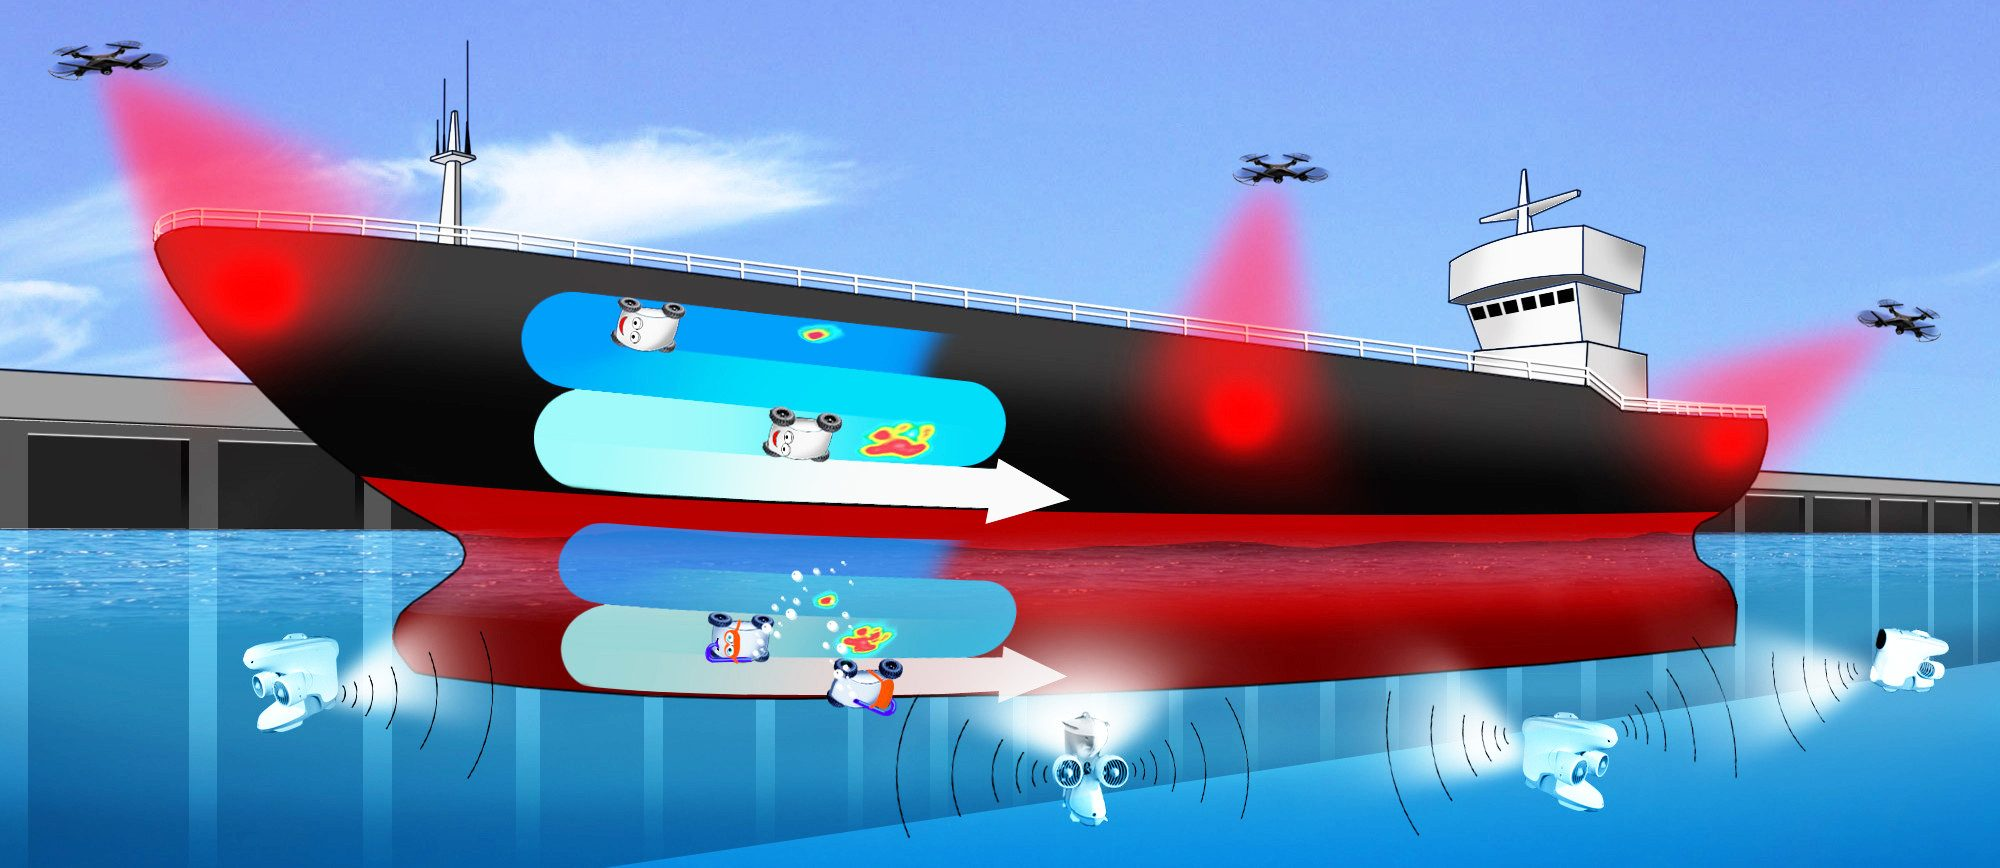
\includegraphics[width=0.8\textwidth]{graphics/Concept-Cartoon-NJ3-e1582812224528.jpg}
				\caption{Projet BugWright2}
			\end{figure}
		\end{frame}
	\section{Objectifs}
		\begin{frame}
			\frametitle{Objectifs}
			Stratégies de navigation multi-robot pour optimiser l'acquisition de données permettant de réaliser la tomographie des structures métalliques
			\begin{itemize}
				\item Recherche bibliographique
				\item Developper algorithmes de navigation
				\item Simulation
				\item Optimisation pour realisation de la tomographie
				\item Coordination entre les robots
				\item Tests sur vrais robots
			\end{itemize}
		\end{frame}
	\section{Environnement Scientifique et Technique}
		\begin{frame}
			\frametitle{Environnement Scientifique et Technique}
			\begin{itemize}
				\item ROS 1
				\item Gazebo
				\item Python, C++
				\item laboratoire CITI, Laboratoire GT-CNRS
			\end{itemize}
		\end{frame}
		\begin{frame}
			\frametitle{Environnement Scientifique et Technique}
			\begin{figure}
				\centering
				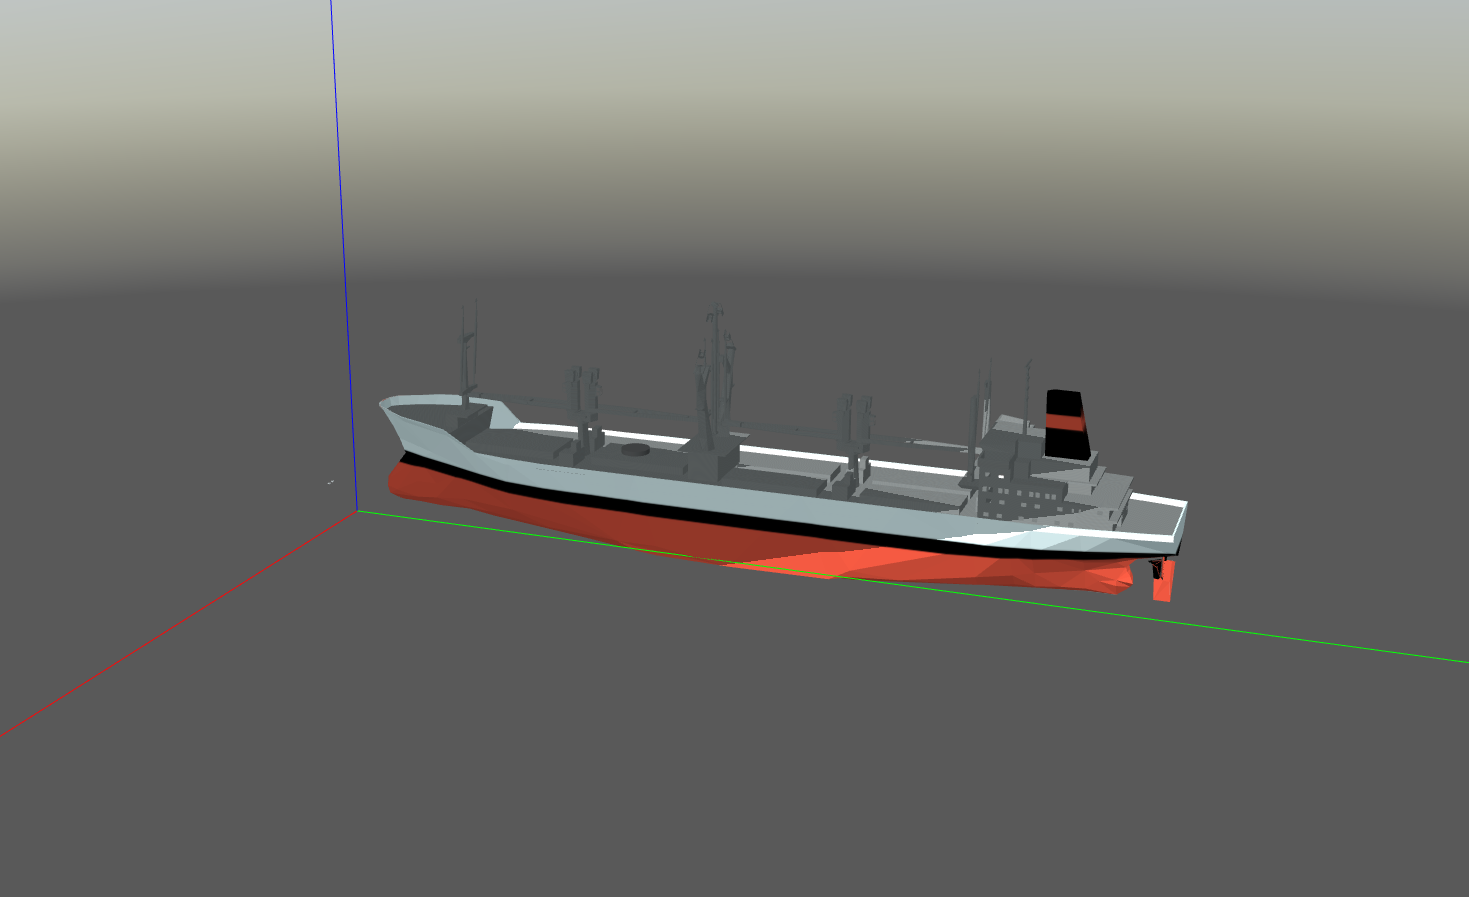
\includegraphics[width=0.8\textwidth]{graphics/boat.png}
				\caption{Gazebo - Modèle de bateau}
			\end{figure}
		\end{frame}
		\begin{frame}
			\frametitle{Environnement Scientifique et Technique}
			\begin{figure}
				\centering
				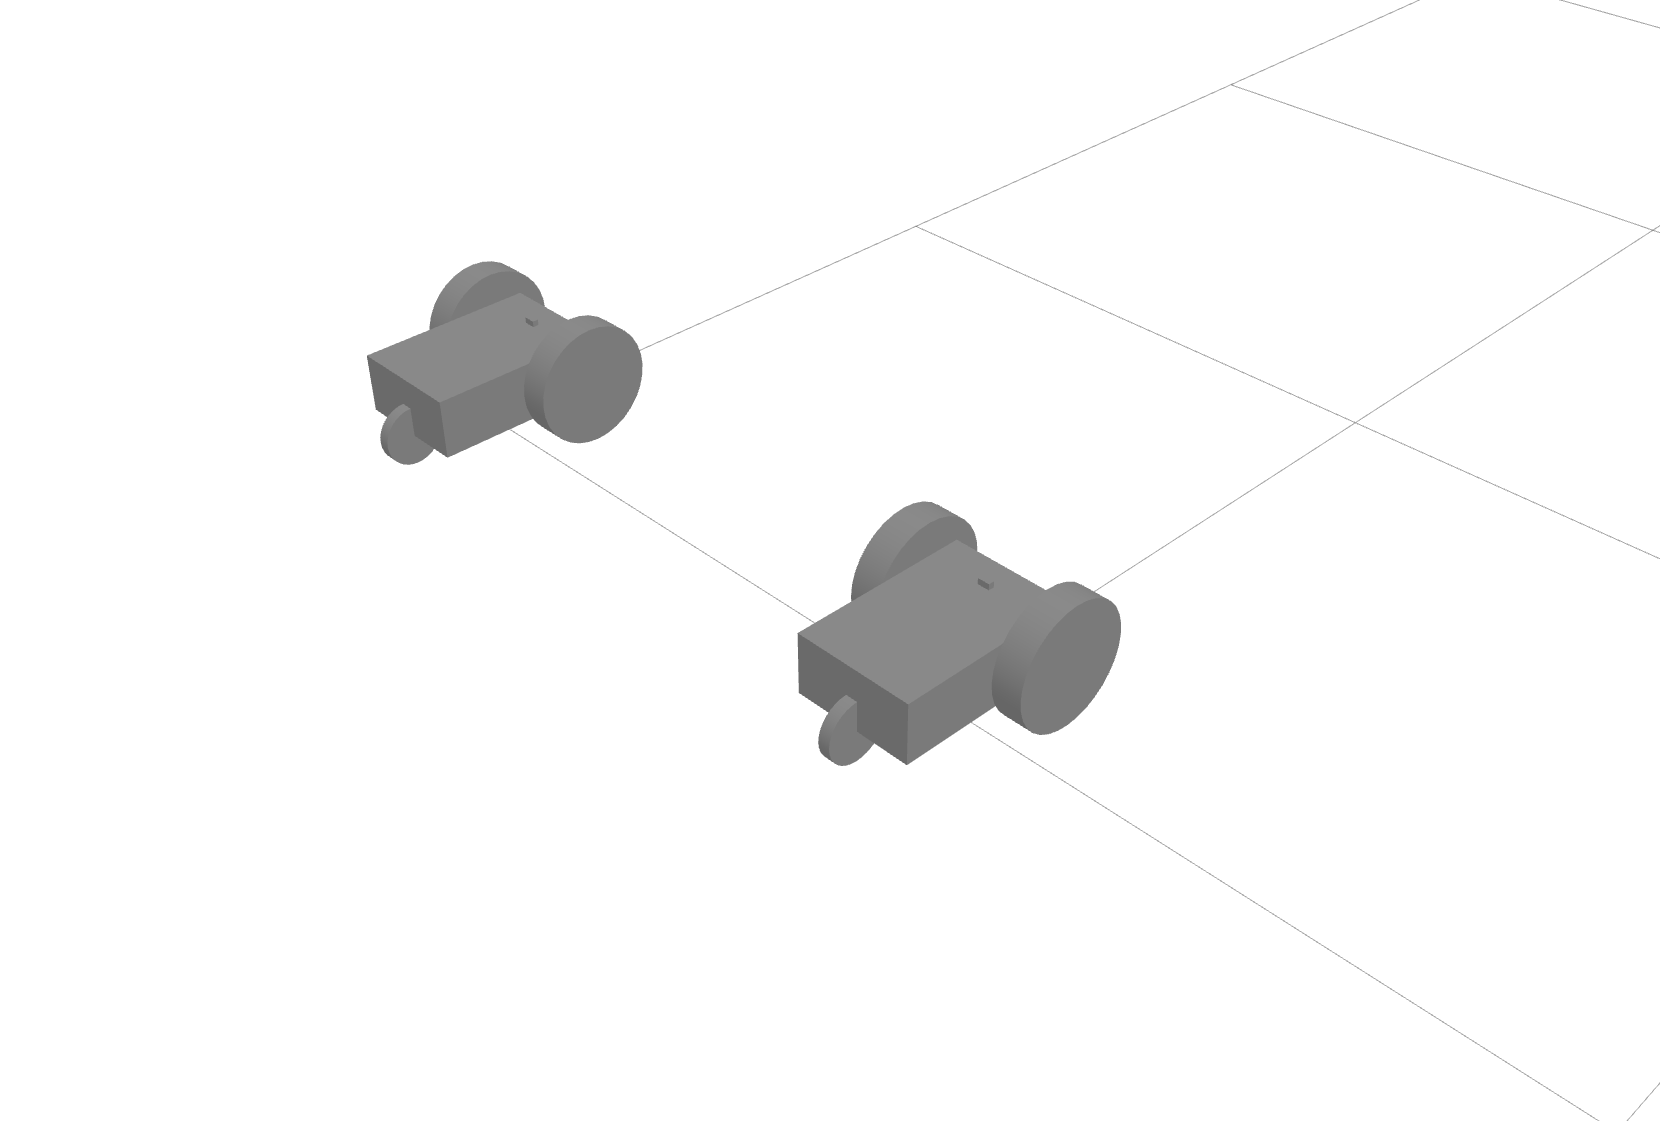
\includegraphics[width=0.8\textwidth]{graphics/crawlers.png}
				\caption{Gazebo - Modèle de crawlers}
			\end{figure}
		\end{frame}
	\section{Organisation}
		\subsection{Livrables}
			\begin{frame}
				\frametitle{Livrables}
				\begin{itemize}
					\item Rapport de projet de fin d'étude
					\item Codes sources
					\item Soutenance orale
				\end{itemize}
			\end{frame}
		\subsection{Planning}
			\begin{frame}
				\frametitle{Planning}
				\begin{itemize}
					\item Recherche bibliographique
					\item Développement des algorithmes
					\item Simulation
					\item Tests expérimentaux
					\item Rapport de fin d'étude
				\end{itemize}
			\end{frame}
	\section{Gestion des Risques}
	    \begin{frame}
	        \frametitle{Gestion des Risques}
	           \begin{itemize}
                \item Incapacité à développer des algorithmes de navigation fiables et précis
                \item Manque de temps pour terminer le projet
                \item Manque de compétences en matière de robotique
                \item Manque de compétences en matière de simulation
    	       \end{itemize}
	    \end{frame}
	\section{Conclusion}
		\begin{frame}
			\frametitle{Conclusion}
			\begin{description}

				\item[Objectif] \hfill \\ Développer des stratégies de navigation multi-robot pour optimiser l'acquisition de données permettant de réaliser une tomographie de la zone à inspecter, avec des ondes ultrasoniques guidées pour réaliser l'inspection de plaques métalliques.
			\end{description}
		\end{frame}
\end{document}
